\opsim~and \altsched~schedulers have adopted two different ways of observing the sky. While the former relies on a greedy algorithm to decide which pointing should be performed (optimisation based on slew-time minimisation, optimal observing conditions - in terms of sky brightness and airmass for instance), the latter scans at the meridian dense areas (pre-defined at the begining of the night) of the sky. Fig. \ref{fig:night_comp} illustrate the area observed at the end of a night for both schedulers. One may observe that \altsched~scans dense area of the sky while regions observed by \opsim~are sparsely populated. It may thus be more difficult to ensure a regular cadence with \opsim~method.

\begin{figure}[!htbp]
  \centering
  \subfigure[OpSim]{\label{fig:opsim_night}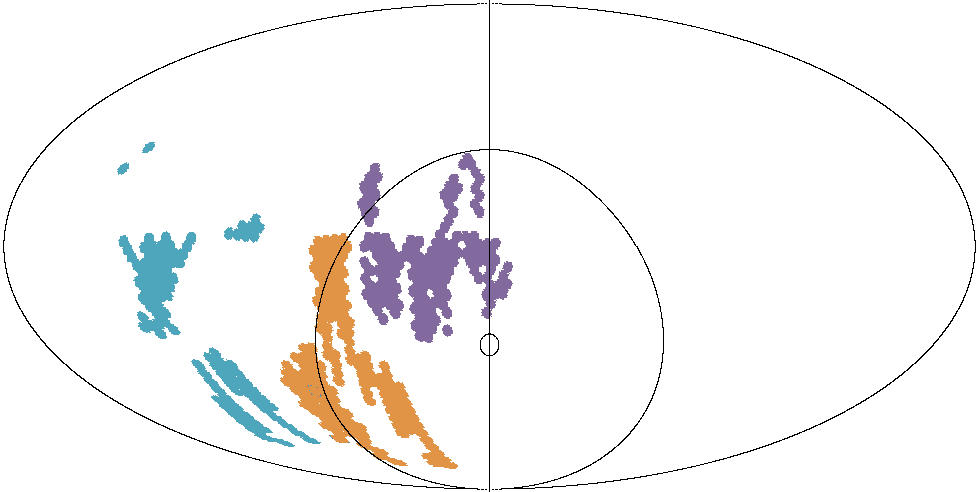
\includegraphics[width=0.8\textwidth]{opsim_vs_altsched/opsim_night.png}}
  \subfigure[altsched]{\label{fig:altsched_night}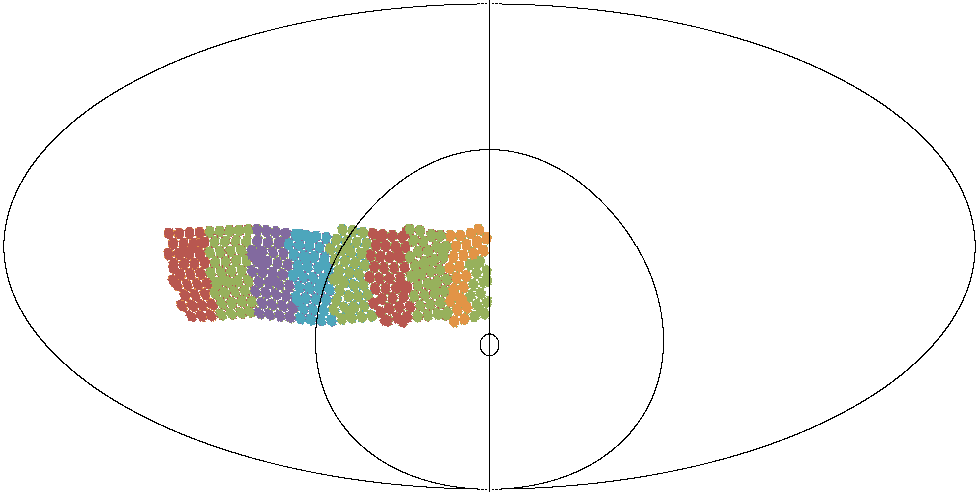
\includegraphics[width=0.8\textwidth]{opsim_vs_altsched/altsched_night.png}}
  \caption{Area coverage at the end of a night for \opsim(top) and \altsched(bottom) schedulers.  Each color point corresponds to a pointing. Colors correspond to the latest filter used.}\label{fig:night_comp}
\end{figure}

One may also observe on Fig. \ref{fig:night_comp} that the filter allocation is quite different between the two schedulers during a night. The number of filter changes per night is indeed higher for \altsched(median value: 12) compared to \opsim(median value: 2) as it can be seen on Fig. \ref{fig:filter_changes}.

\begin{figure}[!htbp]
  \begin{center}
    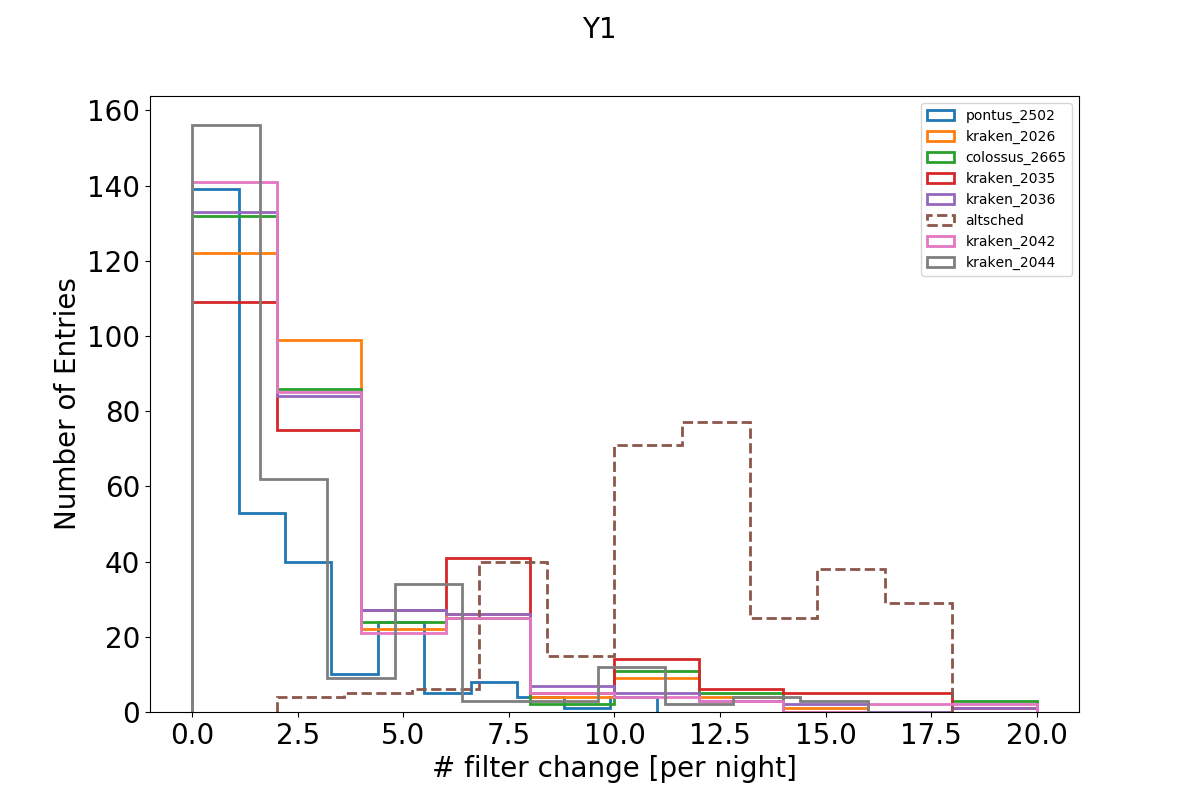
\includegraphics[width=0.6\textwidth]{opsim_vs_altsched/filter_changes.png}
    \caption{Number of filter changes per night (first year of the survey) for some of the observing strategies considered in this work.}\label{fig:filter_changes}
    \end{center}
\end{figure}
